The \textit{Differential Enriched Scan 2} is an R \cite{Ihaka1996} tool developed for detecting epigenomic signal in order to facilitate the Differential Enrichment of the signal between two or more biological conditions.

The package uses Bioconductor \cite{Gentleman2004} data structures and methods every time it was possible, and it is available on Bioconductor since the version 3.7.

It's organized in three main steps. 
A peak caller, which is a standard moving window scan that compares the counts within a sliding window to the counts in a larger region outside the window, using a simple Poisson likelihood (no overdispersion estimation) and providing a final score for each detected peak. 

The filtering step is aimed to determine if a peak is a "true peak" on the basis of its replicability in other samples. To do so, this step is based on a double user-defined threshold, one on the peak score and one on the number of samples.


Finally, the third step produces a counts matrix where each column is a sample and each row a filtered peak computed in the filtering step. The value of the matrix cell is the number of reads for the peak in the sample.

\begin{figure}[H]
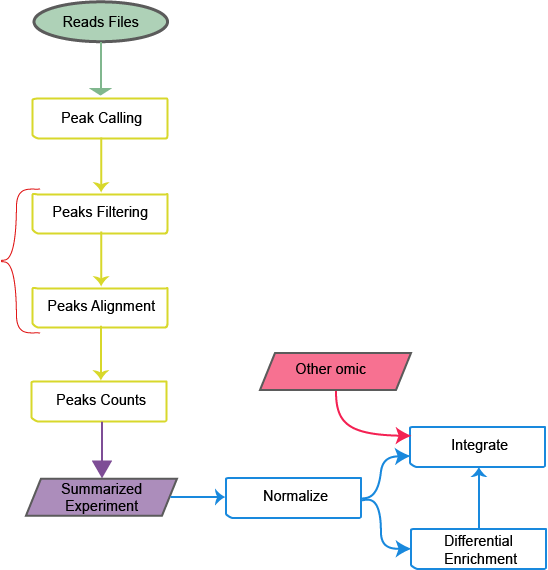
\includegraphics[width=\textwidth,height=\textheight,keepaspectratio]{img/descan2/flow.png}
\caption[DEScan2 workflow]{A differential enrichement flow representation. DEScan2 steps are highlighed in yellow.}
\label{fig:descan2flow}
\centering
\end{figure}

The so produced counts matrix, as illustrated in the figure \ref{fig:descan2flow}, is useful both for doing differential enrichment between the conditions and for integrating the epigenomic data with other -omic data types.

